\setcounter{page}{44}
\newgeometry{top=0cm, bottom=1.8cm, left=3.3cm, right=3.5cm} 

\begin{multicols*}{2}
\begin{figure}[H]
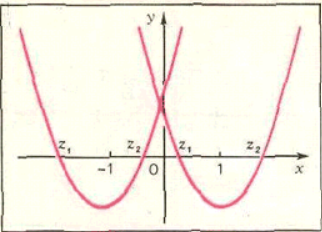
\includegraphics{images/kvant_img.png}
    \caption*{Рис. 3.}
    \label{fig:kv_img}
\end{figure}
\vspace{0.5cm}
\noindent
Сопоставив его с первым ограничением на $m$, получим
$-16/7 \leqslant m < \linebreak < -10/7$.
График нашей параболы при таких значениях m изображен
на риснуке 2. Ее ветви направлены вниз, а корни будут
лежать в интервале $(2, 5)$ тогда и только тогда, когда
$f(2) < 0$ и $f(5) < 0$, то есть
\centerline{$$4 + 2m < 0,\space\space\space25 + 14m < 0$$.}
Отсюда $m < -2$. Окончательно $-16/7 \leqslant m < -2$

З а д а ч а 3 (МАИ, 1970). \textit{При каких действительных
значениях k одно из действительных решений системы}
\begin{equation*}
  \begin{cases*}
    x + y = 2 (k + 1), & \mbox{\raggedright{(2)}}
    \\
    xy = k^2 + 3k - 1 & \mbox{\raggedright{(3)}}
  \end{cases*}
\end{equation*}

\noindent
\textit{удовлетворяет условию $|x| < 1$, $|y| > 1$}?

Наряду с системой $(2)$, $(3)$ естественно рассмотреть
соответствующее ей квадратное уравнение
\mbox{\centerline{$z^2 - 2(k + 1)z + k^2 + 3k - 1 = 0$. (4) }}
\noindent
Оно тесно связано с данной системой, решения которой
получаются с  корней $z_1$ и $z_2$ уравнения $(4)$:
\mbox{$(z_1, z_2)$, $(z_2, z_1)$}.

Легко переформулировать задачу для уравнения (4):
\textit{при каких действительных k один из действительных корней
уравнения $(4)$ находится в интервале $(-1, 1)$, а другой корень
расположен вне этого интервала}.

Так как у квадратного трехчлена $(4)$ должны существовать два различных
действительных корня, то $D > 0$, и график левой части
уравне-
\columnbreak

ния $(4)$ - парабола, пересекающая ось $z$ в двух различных точках
$z_1$ и $z_2$ $(z_1 < z_2)$.

Условию задачи удовлетворяет только такое расположение
корней квадратного трехчлена, когда один из них лежит внутри
интервала $(-1,\linebreak1)$, а другой вне этого
интервала (рис. 3). Если перевести это на формальный язык, то получим
такие системы:
\begin{alignat*}{2}
  \begin{cases*}
    z_1 < -1,
    \\
    -1 < z_2 < 1;
  \end{cases*} & 
  \begin{cases*}\tag{5}
    -1 < z_1 < 1,\\
    z_2 > 1;
  \end{cases*}
\end{alignat*}
\noindent
Чисто технические трудности, возникающие при их решении,
неоправдвнно велики. Изучение же геометрической картины
может подсказать нам менее громоздкий прием.
Нетрудно заметить, что парабола расположена одним
из тех способов, которые изображены на рисунке 3, тогда
и только тогда, когда значения многочлена $f(z)$,
стоящего в левой части $(4)$, в точках $-1$ и $1$ имеют
разные знаки, то есть
\begin{equation}\tag{6}
  f(-1) f(1) < 0.
\end{equation}
\noindent
В самом деле, пусть значение \textit{k} удовлетворяет условию задачи.
Тогда уравнение $(4)$ имеет два действительных корня.
Если один из корней совпадает с $-1$ или $1$, то левая часть
неравенства $(6)$ обращается в нуль. Исключим эти варианты из дальнейшего рассмотрения.

Составим теперь таблицу знаков значений $f(-1) f(1)$ для возможных случаев расположения
$z_1$ и $z_2$ относительно интервала $(-1, 1)$
\newline
$(z_1 < z_2)$

\vspace{0.5cm}
\tiny
{
\centering
\begin{tabular}{ c | c | c | c }
  & & & \\
  & $z_2 < -1$ & $-1 < z_2 < 1$ & $z_2 > 1$ \\
  & & & \\
  \hline
  $z_1 < -1$ & $(+)(+)=+$ & $(-)(+)=-$ & $(-)(-)=+$ \\
  $-1 < z_1 < 1$ & $-$ & $(+)(+)=+$ & $(+)(-)=-$ \\
  $z_1 > 1$ & $-$ & $-$ & $(+)(+)=+$ \\
  & & & \\
\end{tabular}
}
\normalsize
\vspace{0.35cm}

Поскольку исчерпаны все возможные варианты,
то одновременно установлена необходимость и достаточность \mbox{условия (6).
Остается решить}
\end{multicols*}
\newgeometry{left=1.5cm, right=1.5cm, top=1.5cm, bottom=1.5cm}